\section{Analyse préliminaire}\label{Section_AnalysePreliminaire}
Afin d'orienter l'approche à adopter par rapport aux tests et hypothèses à utiliser, il faut d'abord faire une analyse préliminaire des données sur lesquelles le travail est effectué. Ainsi, il s'agit de décrire de façon qualitative les données qui sont utilisées afin de bien interpréter les résultats. Puis, il faut analyser certaines statistiques descriptives afin de voir s'il y a des troncatures ou des censures. Également, une analyse graphique avec les fonctions de densité, les fonctions cumulatives et les fonctions d'excès moyen permettent d'identifier les lois qui sont susceptibles de donner de bons résultats. Finalement, il est possible d'approfondir l'analyse graphique en comparant certains graphiques de quantiles à quantiles (\textit{QQplots}) afin de confirmer les hypothèses soulevées.\\

Pour ce travail, les trois bases de données étudiées sont \texttt{norwegianfire} et \texttt{secura} du \textit{package} \texttt{Reins}, ainsi que \texttt{danish} du \textit{package} \texttt{CASdataset}. Tandis que les deux premières sont analysé dans \cite{norwegianfireEtSecura}, \texttt{danish} est étudié dans \cite{Danish}.\\ 

La présente section présente donc une courte description de chacune d'elles.
	\subsection{\texttt{norwegianfire}}
		Cette base de données est accessible via la commande \texttt{R} \texttt{data("norwegianfire")} ou via \url{http://lstat.kuleuven.be/Wiley}. Il s'agit d'une compilation des pertes relatives aux incendies de forêt ayant eu lieu en Norvège pendant la période de 1972 à 1992.\\ 
		
		À la lecture de ces données, il est important d'observer que les pertes retenues sont supérieures à $500\,000$ couronnes norvégiennes. Par conséquent, on tient compte de cette information en conditionnant.\\
		
		À noter qu'aucune mention n'est faite au sujet d'un éventuel ajustement pour l'inflation. Dans le cadre de ce travail, il est présumé qu'un ajustement est déjà effectué.
		
		\paragraph{Analyse de la fréquence:}
			Afin de procéder à l'analyse préliminaire, l'illustration \ref{Graph_Freq_NorvFire} présente un histogramme du nombre de sinistre sur une base annuelle et la fonction de répartition empirique du nombre de sinistres durant la période de 1972 à 1992.
			
			\begin{figure}[H]
			\centering
				\begin{subfigure}[b]{0.45\textwidth}
					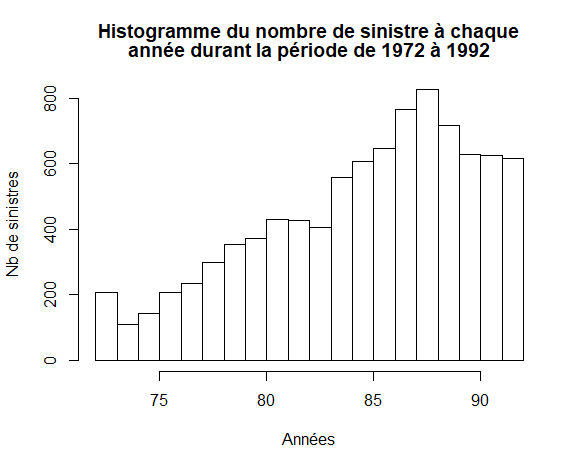
\includegraphics[scale=0.45]{Graphiques/HistFreqNorwegianfire} 
					\caption{} \label{HistFreqNorwegianfire}
				\end{subfigure}
				\begin{subfigure}[b]{0.4\textwidth}
					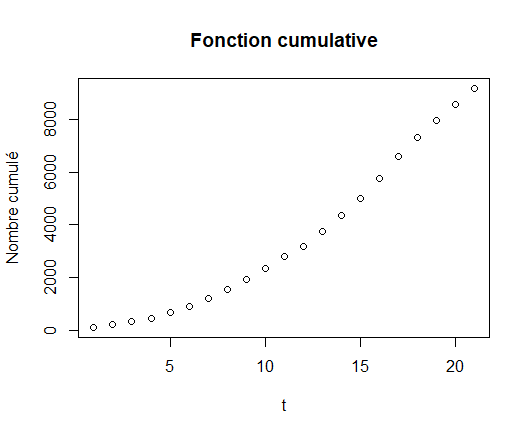
\includegraphics[scale=0.45]{Graphiques/Graph_Norwegianfire_FreqCumul} 
					\caption{} \label{Graph_Norwegianfire_FreqCumul}
				\end{subfigure}
				\renewcommand{\figurename}{Illustration}
				\caption{Analyse de la fréquence pour \texttt{norwegianfire}.}\label{Graph_Freq_NorvFire}
			\end{figure}
		
			Lorsque l'on regarde l'illustration \ref{HistFreqNorwegianfire}, on voit que l'intensité de la fréquence semble augmenter d'année en année. Cependant, entre les années 1986 et 1988, il s'est produit un événement qui a stoppé cet accroissement. En effet, en regardant l'analyse qui a été faite par la European Commission\footnote{\url{http://effis.jrc.ec.europa.eu/media/cms_page_media/40/Forest_fires_in_Europe_Middle_east_and_North_Africa_2016_final_pdf_JZU7HeL.pdf}}, aux page 36-38, on peut y voir que plusieurs mesures ont été prises par la Norvège afin de réduire le nombre d'incendies de forêt. De plus, en regardant l'illustration 33b de la dite analyse, on voit que le nombre de sinistres tend à redescendre. À noter que l'échelle de ce graphique est biaisée du fait que les méthodes statistiques avaient été changées. C'est pour cette raison que l'on voit une forte hausse en 2016; le biais a été corrigé à ce moment. En revanche, ce qui est intéressant de remarquer, c'est la tendance descendante jusqu'en 2015.\\
			
			Or, considérant que l'objectif de ce travail est de créer un modèle de prédiction du nombre de sinistres pour les années à venir, il faut que le processus utilisé soit représentatif des tendances futures. Pour cette raison, il est avisé de considérer un processus de Poisson homogène dont l'intensité serait la moyenne des trois dernières années de la base de données \texttt{norwegianfire}, soit 622 sinistres.
			
			\paragraph{Analyse de la sévérité:}
			Du point de vue de la sévérité, en regardant l'illustration \ref{Hist_SeverNorwegianFire}, on observe que les données extrêmes nuisent à la lecture de la distribution globale de la sévérité. L'illustration \ref{Hist_SevNorwegianFire2} permet, quant à lui, de remédier à ce problème. Ainsi, on observe que le logarithme des montants de sinistre semble suivre une loi exponentielle.
			
			\begin{figure}[H]
				\centering
				\begin{subfigure}[b]{0.3\textwidth}
					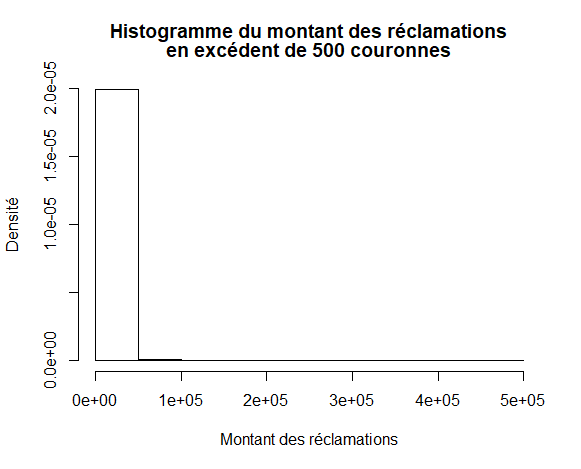
\includegraphics[scale=0.35]{Graphiques/Hist_SeverNorwegianFire} 
					\caption{} \label{Hist_SeverNorwegianFire}
				\end{subfigure}
				\begin{subfigure}[b]{0.3\textwidth}
					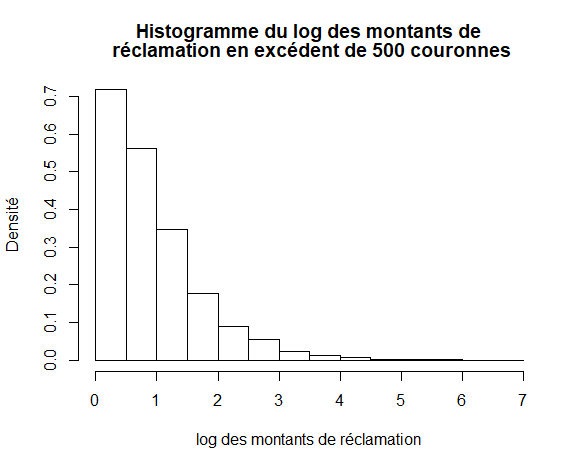
\includegraphics[scale=0.35]{Graphiques/Hist_SevNorwegianFire2}
					\caption{} \label{Hist_SevNorwegianFire2}
				\end{subfigure}
				\begin{subfigure}[b]{0.3\textwidth}
					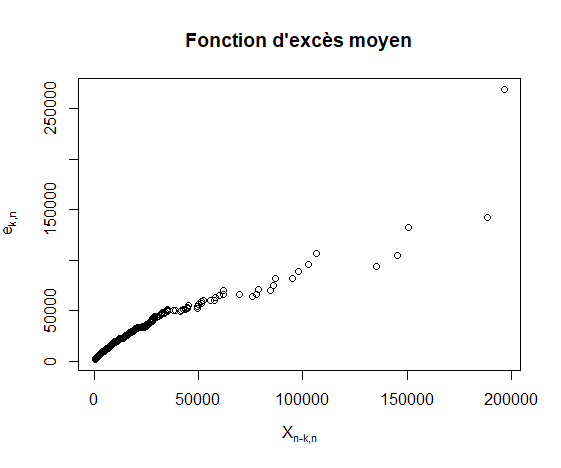
\includegraphics[scale=0.35]{Graphiques/Graph_Norwegianfire_MeanExcess} 
					\caption{} \label{Graph_Norwegianfire_MeanExcess}
				\end{subfigure}
				\renewcommand{\figurename}{Illustration}
				\caption{Analyse de la sévérité pour \texttt{norwegianfire}.} \label{Graph_Sev_NorvFire2}
			\end{figure}
			
			D'ailleurs, l'illustration \ref{QQplot_Pareto_NorweginaFIre} vient confirmer cette observation.
			
			\begin{figure}[H]
			\begin{center}
					\begin{subfigure}[H]{0.45\textwidth}
						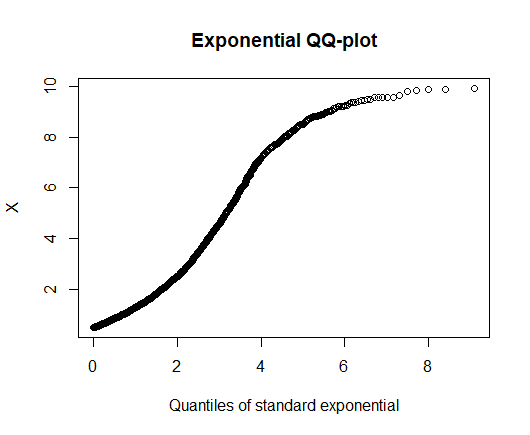
\includegraphics[scale=0.45]{Graphiques/QQplot_Exp_NorwegianFire}
						\caption{} \label{QQplot_Exp_NorwegianFire}
					\end{subfigure}
					\begin{subfigure}[H]{0.4\textwidth}
						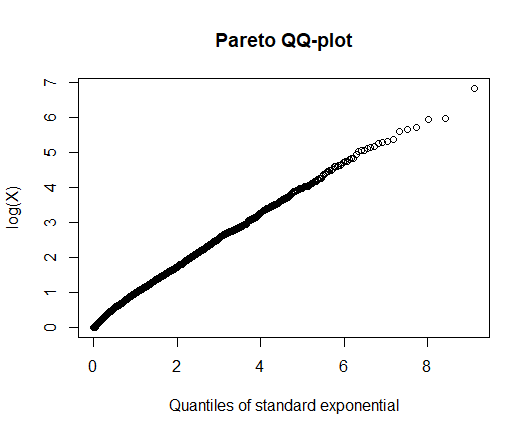
\includegraphics[scale=0.45]{Graphiques/QQplot_Pareto_NorweginaFIre}
						\caption{} \label{QQplot_Pareto_NorweginaFIre}
					\end{subfigure}
				\renewcommand{\figurename}{Illustration}
				\caption{\textit{QQplots} préliminaires pour \texttt{norwegianfire.}}
				\end{center}
			\textbf{Remarque:}\textit{Ces graphiques sont produits avec les commandes \texttt{R} provenant du \textit{package} \texttt{Reins: ExpQQ et ParetoQQ}.}
			\end{figure}
			En effet, l'illustration \ref{QQplot_Exp_NorwegianFire} montre le graphique des quantiles d'une loi exponentielle standard vis-à-vis des quantiles empiriques liés aux montants de sinistre tandis que l'illustration \ref{QQplot_Pareto_NorweginaFIre} compare les quantiles de la même loi exponentielle vis-à-vis du logarithme des données empiriques. 
			
			\begin{Proposition}\label{Propo_Pareto}
				Soit $X$, une variable aléatoire modélisant les montants de sinistre, \\si $\ln X \sim Exponentielle(\lambda)$, alors $X\sim Pareto(\lambda)$.
			\end{Proposition}
			
			\begin{proof}[Démonstration]
				Posons $Y=\ln X \sim Exp(\lambda)$. Alors, on a 
				$$
				\bar{F}_Y(y) = e^{-\lambda y} = e^{-\lambda \ln x} = x^{-\lambda} = \bar{F}_X(x),\: x\geq 1.
				$$
				On obtient alors la fonction de répartition d'une loi de Pareto de type 1 avec un paramètre de forme égal à $\lambda$ et le domaine débute à 1.
			\end{proof}

			Donc, on peut déduire de la proposition \ref{Propo_Pareto} qu'un modèle basé sur une loi de Pareto est un choix judicieux pour modéliser la sévérité de la base de données de la \texttt{norwegianfire}.\\
			
			Finalement, du point de vue des statistiques descriptives, le tableau \ref{Stats_Norwegianfire} résume les principaux points intéressants pour la sévérité des sinistres.
			
			\begin{table}[H]
				\begin{center}
				\begin{tabular}{ccccccc}
					Min.& $1^{er}$ Qu.	&	Médiane	&	Moyenne	&	$3^e$ Qu	&	Max.	&	écart type \\
					\hline
					500	&	700			&	1\,020	&	2\,217	&	1\,800		&	465\,400	&	7\,760
				\end{tabular}
				\renewcommand{\tablename}{Tableau}
				\caption{Statistiques descriptives de \texttt{norwegianfire}.}\label{Stats_Norwegianfire}
				\end{center}
			\end{table}
		
			Les statistiques du tableau \ref{Stats_Norwegianfire} sont utiles lors de l'établissement d'un point de départ dans l'algorithme d'estimation des paramètres avec la méthode du maximum de vraisemblance.
			
	\subsection{\texttt{secura}}
		Toujours dans le \textit{package} \texttt{Reins}, la base de données \texttt{secura} comporte des montants de perte en assurance automobile venant de plusieurs pays d'Europe pendant la période de 1988 à 2001. Ces montants sont en excédant de 1\,200\,000 euros et sont ajustées pour l'inflation.
		
		\paragraph{Analyse de la fréquence:}
		De façon similaire à l'analyse précédente, l'illustration \ref{Hist_freq_Secura} est un histogramme sur le nombre annuel de sinistres dans la période de 1988 à 2001 et l'illustration \ref{Graph_Secura_FreqCumul} présente la fonction de répartition empirique de ce dénombrement.
		
		\begin{figure}[H]
			\begin{center}
				\begin{subfigure}[b]{0.45\textwidth}
					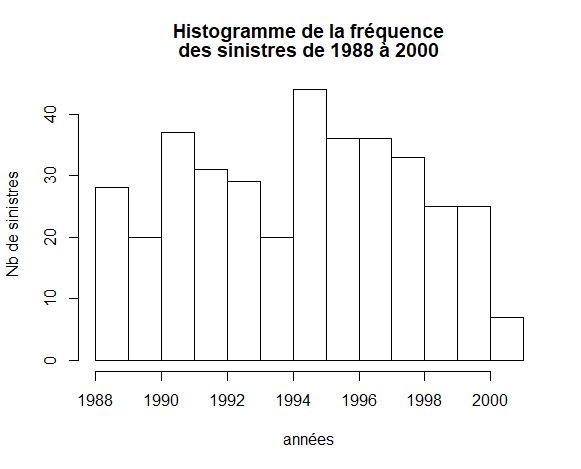
\includegraphics[scale=0.45]{Graphiques/Hist_freq_Secura} 
					\caption{} \label{Hist_freq_Secura}
				\end{subfigure}
				\begin{subfigure}[b]{0.4\textwidth}
					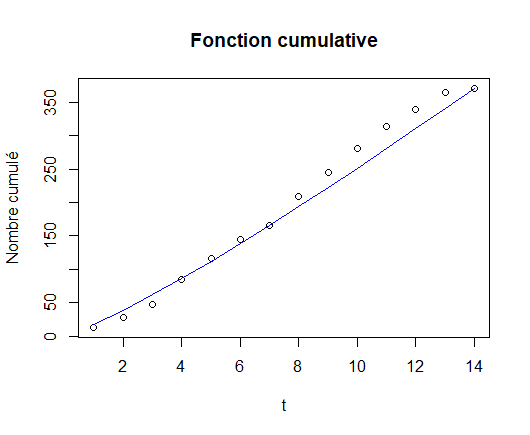
\includegraphics[scale=0.45]{Graphiques/Graph_Secura_FreqCumul} 
					\caption{} \label{Graph_Secura_FreqCumul}
				\end{subfigure}
			\renewcommand{\figurename}{Illustration}
			\caption{Analyse de la fréquence pour \texttt{secura}.}\label{Graph_freq_Secura}
			\end{center}
		\end{figure}
	
		À la lecture de l'illustration \ref{Hist_freq_Secura}, on voit que la fréquence des sinistres semblent avoir une tendance cyclique sur 4 ans. Cependant, selon le contexte, cela est très peu probable puisque il est illogique de penser que le nombre d'accidents diminuerait à tous les quatre ans pour ensuite remonter d'un coup à un niveau plus élevé. Par contre, suite à la recherche de données complémentaires sur l'internet, aucune information ne nous permet de contredire ces résultats. Pour cette raison, on ne peut assumer que ces informations sont fausses \textit{a posteriori} et elles doivent être considérer comme tel dans l'analyse de la fréquence.\\
		
		À ce moment, il est approprié de tester un processus de Poisson non-homogène avec une intensité périodique afin d'étudier ce comportement. Par ailleurs, en regardant l'illustration \ref{Graph_Secura_FreqCumul}, on voit que cette périodicité n'est peut être pas significative puisque les écarts entre les points et la droite qui est tracée ne sont pas très grands. Afin de comparer ces deux modèles, il est nécessaire de procéder au test du ratio de maximum de vraisemblance pour valider s'il y a réellement un gain à avoir un modèle plus complexe par rapport à un processus de Poisson homogène.
		
		\paragraph{Analyse de la sévérité:}
		Au niveau de l'analyse de la sévérité, en regardant l'illustration \ref{Hist_Severite_Secura}, une loi de forme exponentielle semble, \textit{a priori}, bien modéliser le corps de la distribution. 
		
		\begin{figure}[H]
		\begin{center}
		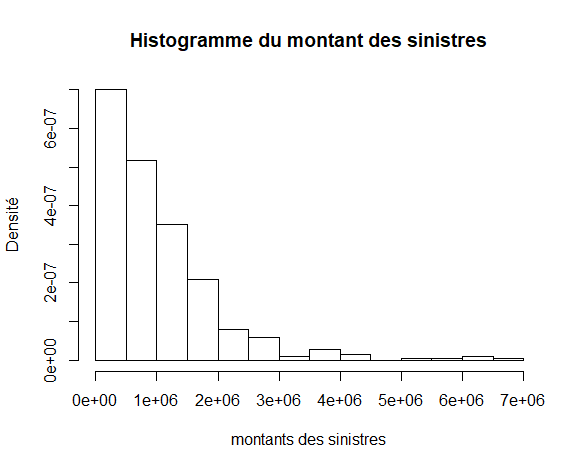
\includegraphics[scale=0.45]{Graphiques/Hist_Severite_Secura} 
		\renewcommand{\figurename}{Illustration}
		\caption{Analyse de la sévérité pour \texttt{secura}.} \label{Hist_Severite_Secura}
		\end{center}
		\end{figure}
		
		L'illustration \ref{QQPlot_Expo_Secura} permet, quant à lui, de confirmer cette hypothèse.
		
		\begin{figure}[H]
			\begin{center}
				\begin{subfigure}[b]{0.45\textwidth}
					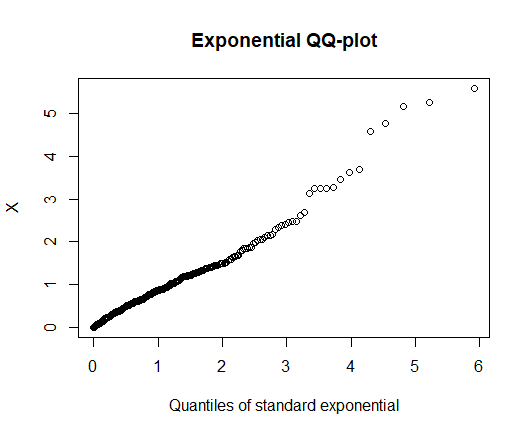
\includegraphics[scale=0.43]{Graphiques/QQPlot_Expo_Secura} 
					\caption{} \label{QQPlot_Expo_Secura}
				\end{subfigure}
				\begin{subfigure}[b]{0.4\textwidth}
					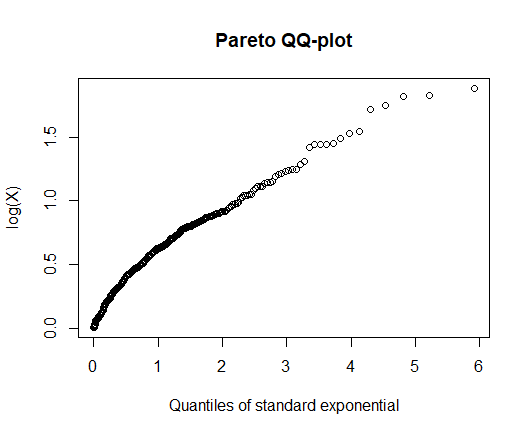
\includegraphics[scale=0.43]{Graphiques/QQplot_Pareto_Secura} 
					\caption{} \label{QQplot_Pareto_Secura}
				\end{subfigure}
				\renewcommand{\figurename}{Illustration}
				\caption{\textit{QQplots} préliminaires pour \texttt{secura}.}
			\end{center}
		\end{figure}
		
		En revanche, en regardant l'illustration \ref{Graph_Secura_MeanExcess}, on voit de façon plus détaillé quelles lois pourraient être utilisées.\\
		
		\begin{figure}[H]
			\begin{center}
			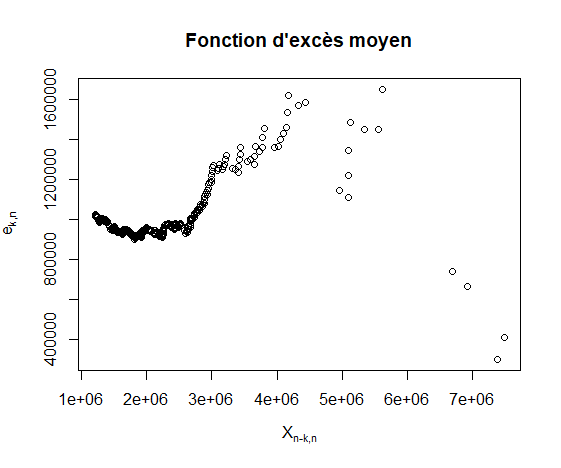
\includegraphics[scale=0.45]{Graphiques/Graph_Secura_MeanExcess} 
			\renewcommand{\figurename}{Illustration}
			\caption{Fonction d'excès moyen pour \texttt{secura}.} \label{Graph_Secura_MeanExcess}
			\end{center}
		\end{figure}
		
		En effet, \cite{Embrechts1994}(p.11-14) font  une analyse de distribution se basant sur la fonction d'excès moyen. Les résultats de cette analyse sont résumés sur l'illustration \ref{Interpretation_Graph_ExcesMoyens}.
		
		\begin{figure}[H]
			\begin{center}
			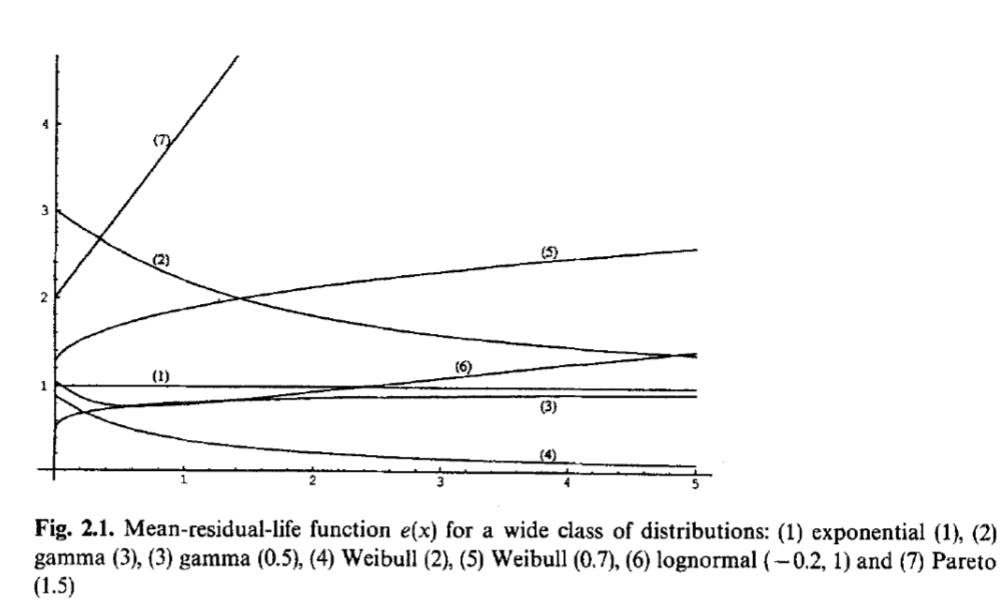
\includegraphics[scale=0.45]{Graphiques/Interpretation_Graph_ExcesMoyens} 
			\renewcommand{\figurename}{Illustration}
			\caption{Embrechts et Schmidli: Détermination de la loi de sévérité en fonction de la fonction d'excès moyen.} \label{Interpretation_Graph_ExcesMoyens}
			\end{center}
		\end{figure}
		
		Ainsi, en observant, le graphique d'excès moyen, nous sommes en mesure de faire une analyse approfondie afin de déterminer de façon analytique quelles lois pourraient être utilisées. De plus,  advenant de devoir faire des raccordements de lois, cet indicateur peut aider, en théorie, à déterminer les valeurs de $X$ où il faut appliquer les points de raccordement.\\
		
		De cette façon, en regardant à nouveau l'illustration \ref{Graph_Secura_MeanExcess}, on peut voir que les deux lois pouvant modéliser le mieux le début de la distribution seraient la loi gamma ou possiblement la loi de Weibull. Puis, un premier raccordement serait fait aux alentours de $2\,900\,000$ \euro. À cette valeur, un raccordement approprié serait fait avec une loi de Pareto afin de bien représenter les valeurs extrêmes. Cependant, la nature des points qui suivent n'est pas claire à ce stade-ci de l'analyse.\\
		
		Néanmoins, plusieurs modèles doivent être testés afin de valider les hypothèses soulevées grâce à la découverte de \cite{Embrechts1994} et pour optimiser la vraisemblance du modèle.\\
						
		Finalement, les statistiques descriptives de la base de données sont présentées dans le tableau \ref{Stats_Secura}.
				
		\begin{table}[H]
			\begin{center}
				\begin{tabular}{ccccccc}
					Min.& $1^{er}$ Qu.	&	Médiane	&	Moyenne	&	$3^e$ Qu	&	Max.	&	écart type \\
					\hline
					1\,208\,000 & 1\,573\,000 & 1\,944\,000 & 2\,231\,000 & 2\,609\,000 & 7\,899\,000 	&	1\,011\,218
				\end{tabular}
				\renewcommand{\tablename}{Tableau}
				\caption{Statistiques descriptives de \texttt{secura}.}\label{Stats_Secura}
			\end{center}
		\end{table}
	
	En regardant ce tableau, on voit que la valeur minimale de l'échantillon est de $1\,208\,000$ \euro. Malgré cette information, pour le présent travail, il est assumé que les données ont bien été tronquées à $1\,200\,000$ \euro\;afin d'être cohérent avec l'analyse descriptive ci-haut.
	
	\subsection{\texttt{danish}}
		La dernière base de données, \texttt{danish}, se trouve dans le \textit{package} \texttt{R CASdataset} avec la commande \texttt{data(danishuni)}. Elle est aussi disponible au lien suivant: \url{http://www.ma.hw.ac.uk/~mcneil/data.html}. Elle a été compilée à la Copenhagen Reinsurance et comprend 2\,167 pertes liées à des incendies au cours de la période de 1980 à 1990. Elle a été ajustée pour inflation et les valeurs sont exprimées en millions de couronnes danoises.\\
		
		Par ailleurs, ce qui distingue cette base de données des deux autres, c'est qu'elle présente les sinistres à chaque jour. Il est donc possible d'avoir une analyse de la fréquence plus approfondie. Malheureusement, pour pouvoir tester un processus de renouvellement, il aurait fallu qu'il n'y ait pas plus d'un événement par jour ou que la périodicité soit exprimé en termes d'heures. Or, comme ce n'est pas le cas, il n'est pas possible de modéliser les temps inter-sinistres adéquatement.
		
		\paragraph{Analyse de la fréquence:}
		Comme pour les deux autres bases de données, l'analyse préliminaire débute avec l'histogramme \ref{Hist_Danish_Frequence} qui présente le nombre de sinistres dans la période de 1980 à 1990, sur une base quotidienne, puis le graphique \ref{Graph_Danish_FreqCumul} qui présente la fonction de répartition  empirique de ce dénombrement.
		
		\begin{figure}[H]
			\begin{center}
				\begin{subfigure}[b]{0.52\textwidth}
					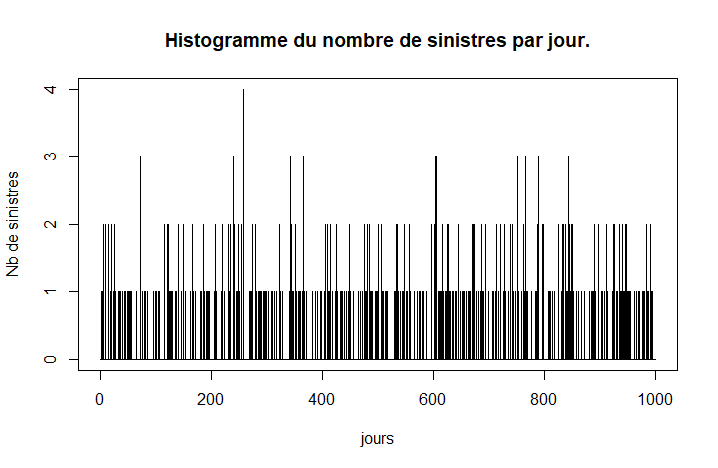
\includegraphics[scale=0.5]{Graphiques/Hist_Danish_Frequence} 
					\caption{} \label{Hist_Danish_Frequence}
				\end{subfigure}
			\begin{subfigure}[b]{0.42\textwidth}
				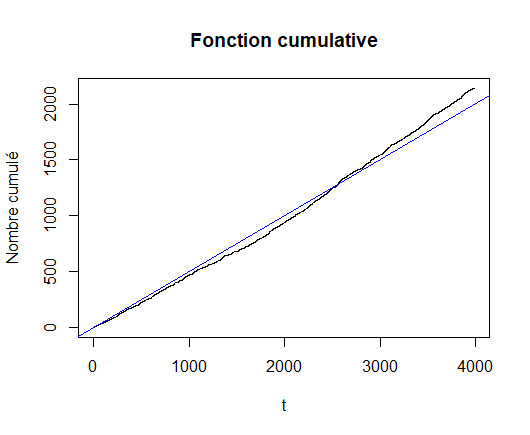
\includegraphics[scale=0.5]{Graphiques/Graph_Danish_FreqCumul} 
				\caption{} \label{Graph_Danish_FreqCumul}
			\end{subfigure}
			\renewcommand{\figurename}{Illustration}
			\caption{Analyse de la fréquence pour \texttt{danish}.}\label{Graph_Freq_Danish}
			\end{center}
		\end{figure}
		
		L'illustration \ref{Graph_Danish_FreqCumul} montre qu'il y a une très légère hausse de l'intensité au fil du temps.\\
		
		Cependant, l'illustration \ref{Graph_CompLimit_PoissHomo} peut laisser croire qu'il s'agit d'un processus de Poisson homogène puisque l'on peut y observer le comportement limite d'un processus de Poisson dont l'intervalle de temps tend vers l'infini.
		
		\begin{figure}[H]
			\begin{center}
			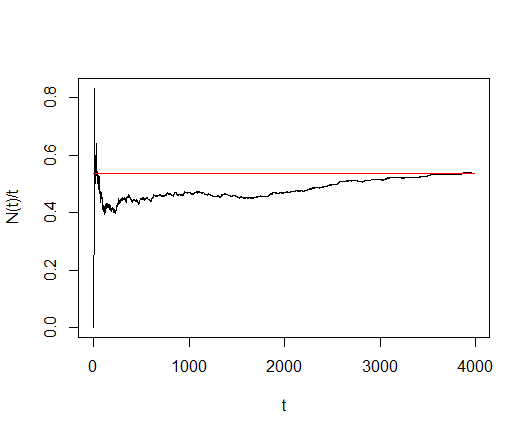
\includegraphics[scale=0.5]{Graphiques/Graph_CompLimit_PoissHomo} 
			\end{center}
			\renewcommand{\figurename}{Illustration}
			\caption{Comportement limite d'un Processus de Poisson.} Lorsque l'intervalle de temps(t) sur lequel un Processus de Poisson est étudié est grand, le nombre de sinistres divisé par l'intervalle de temps sur lesquels ces sinistres ont été observés tend vers le taux d'intensité du Processus.(\cite{Mikosch_PoissProcess2009}, p.56-60).\label{Graph_CompLimit_PoissHomo} 
		\end{figure}
	
		Comme pour la base de données \texttt{secura}, le test du ratio de vraisemblance permet de déterminer si l'augmentation est significative ou si un modèle de Poisson homogène capture réellement le comportement de ces données.
		
		\paragraph{Analyse de la sévérité:}
		Pour ce qui est de la sévérité, en regardant les graphiques \ref{Hist_Danish_Severite} et \ref{Hist_Danish_LogSeverite}, un comportement similaire à celui de la base de données \texttt{norwegianfire} est observable. En effet, le logarithme des montants de sinistre semble suivre une loi exponentielle. L'utilisation d'un modèle basé sur la loi de Pareto semble donc aussi adéquat.
		
		\begin{figure}[H]
			\begin{center}
			\begin{subfigure}[b]{0.3\textwidth}
				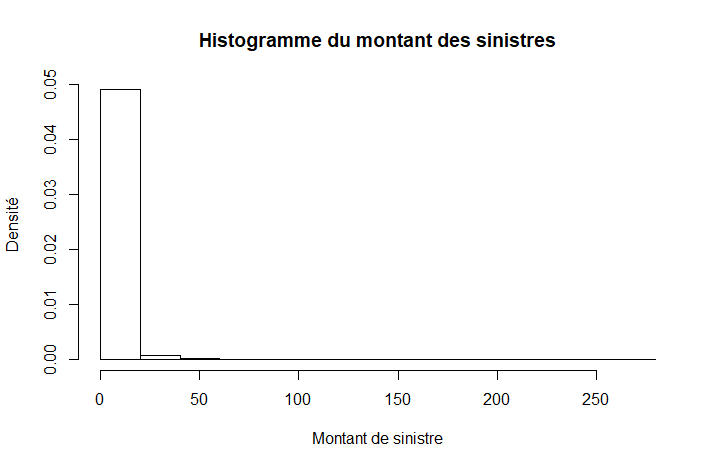
\includegraphics[scale=0.35]{Graphiques/Hist_Danish_Severite} 
				\caption{} \label{Hist_Danish_Severite}
			\end{subfigure}
			\begin{subfigure}[b]{0.3\textwidth}
				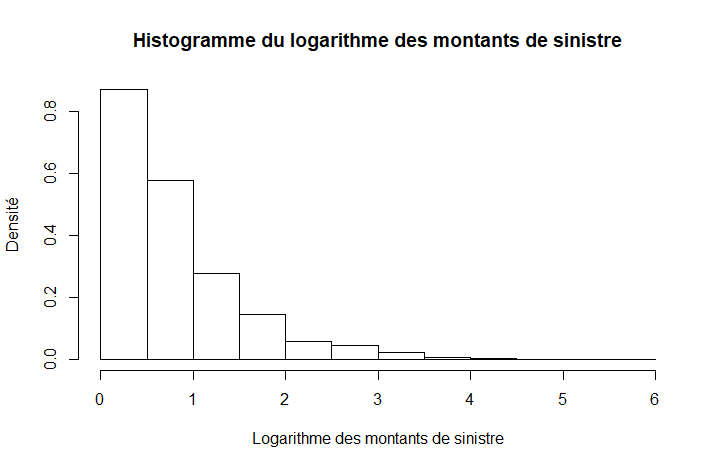
\includegraphics[scale=0.35]{Graphiques/Hist_Danish_LogSeverite} 
				\caption{} \label{Hist_Danish_LogSeverite}
			\end{subfigure}
			\begin{subfigure}[b]{0.3\textwidth}
				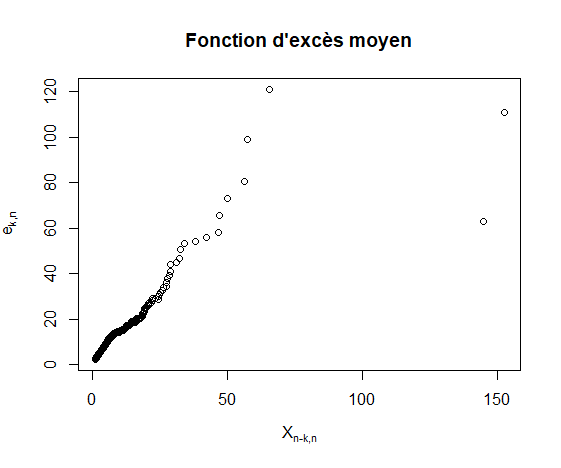
\includegraphics[scale=0.35]{Graphiques/Graph_Danish_MeanExcess} 
				\caption{} \label{Graph_Danish_MeanExcess}
			\end{subfigure}
			\renewcommand{\figurename}{Illustration}
			\caption{Analyse de la sévérité pour \texttt{danish}.}\label{Hist_Danish}
			\end{center}
		\end{figure}
		
		De plus, l'illustration \ref{QQplot_Pareto_Danish} vient confirmer cette observation.
		
		\begin{figure}[H]
			\begin{center}
				\begin{subfigure}[b]{0.5\textwidth}
					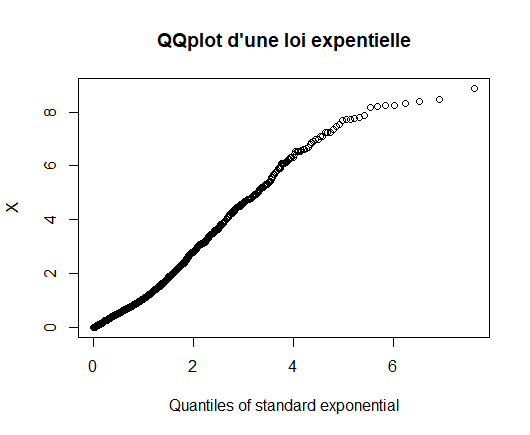
\includegraphics[scale=0.45]{Graphiques/QQplot_Exp_Danish} 
					\caption{Fréquence} \label{QQplot_Exp_Danish}
				\end{subfigure}
				\begin{subfigure}[b]{0.4\textwidth}
					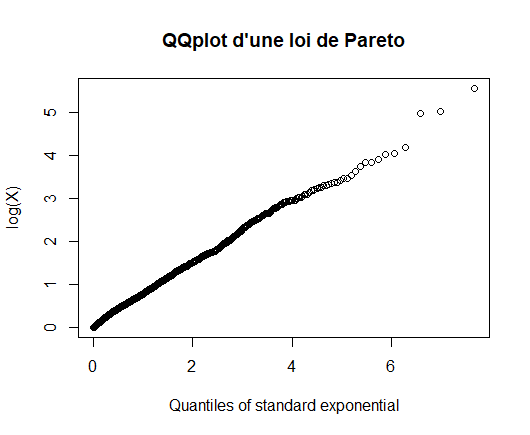
\includegraphics[scale=0.45]{Graphiques/QQplot_Pareto_Danish} 
					\caption{Sévérité} \label{QQplot_Pareto_Danish}
				\end{subfigure}
				\renewcommand{\figurename}{Illustration}
				\caption{\textit{QQplots} préliminaires pour \texttt{danish}.}
			\end{center}
		\end{figure}
		
		En regardant le tableau \ref{Stats_Danish}, on voit que la valeur minimale est d'un million de couronnes danoises. Donc, il faut conditionner sur cette valeur où se trouve la troncature.
		
		\begin{table}[H]
			\begin{center}
				\begin{tabular}{ccccccc}
					Min.& $1^{er}$ Qu.	&	Médiane	&	Moyenne	&	$3^e$ Qu	&	Max.	&	écart type \\
					\hline
					1,000  & 1,321 &  1,778 &  3,385 &  2,967 & 263,300  	&	8,507
				\end{tabular}
				\renewcommand{\tablename}{Tableau}
				\caption{Statistiques descriptives de \texttt{danish}.}\label{Stats_Danish}
			\end{center}
		\end{table}		
		